%!TEX root = ../DigPro2.tex
\section{Image Pattern Classification\buch{Ch. 12}\buchSeite{903-994}}
\begin{itemize}
\item Recognition of \emph{individual} image regions called \emph{object} or \emph{pattern}
\item Concept of ``learning'' from sample patterns
\end{itemize}

\subsection{Patterns and Pattern Classes\buchSeite{906}}
\begin{itemize}
	\item A \emph{pattern} is an arrangement of descriptors
		(as in Section \ref{sec:featureExtraction}) in pattern classification
		called \emph{features}.
	\item A \emph{pattern class} is a set of patterns, denoted $\omega_1, \omega_2, ..., \omega_W$, where W is the number of classes
	\item The goal is to assign a given patter into a class
\end{itemize}

\subsubsection{Vectors\buchSeite{906}}
\begin{itemize}
	\item Used for quantitative descriptors
	\item every dimension contains the numerical value of a descriptor
	\item $\mathbf{x} =
		\begin{bmatrix}
			x_1 \\
			x_2 \\
			\vdots \\
			x_n \\
		\end{bmatrix}
		 = (x_1, x_2, \ldots, x_n)^T $
\end{itemize}
Example: Classifying flowers based on petal length and width into one of three classes.

\subsubsection{Structural Patterns\buchSeite{908}}
Structural information can be captured in strings. Example in Section \ref{sec:boundaryFeatureDescriptors} \nameref{sec:boundaryFeatureDescriptors}
\begin{itemize}
	\item Connectivity patterns (order is important)
	\item Compact description, better than sampling into a feature vector
\end{itemize}

\paragraph{Tree\buchSeite{910}}
If there is hierarchy then a descriptor which is based on a tree structure
should be used.

\subsection{Pattern Classification by Prototype Matching\buchSeite{910}}
\paragraph{Minimum-distant Classifier\buchSeite{910}}
The core of decision theory $d_i(\mathbf{x})$ defined for each class $\omega_i$.
These are not known and finding them is the main goal. \\

A class $\omega_i$ is selected if
\begin{align*}
d_i(\mathbf{x}) > d_j(\mathbf{x}) && j=1,2, \cdots, W; j \neq i
\end{align*}
The interesting parts are decision boundaries between classes
\begin{align*}
	d_i(\mathbf{x}) - d_j(\mathbf{x}) = 0
\end{align*}
For two classes, a single discriminant function can be introduced
\begin{align*}
	d_{ij}(\mathbf{x}) = d_i(\mathbf{x}) - d_j(\mathbf{x}) = 0
\end{align*}

\subsubsection{Matching}
Each class is represented by prototypes.
A vector $x$ belongs to the class with the shortest distance.

\paragraph{Minimum-distance classifier}
The mean vector of a class is a powerful prototype vector.
\begin{align*}
	\mathbf{m}_j = \frac{1}{n_j} \sum_{\mathbf{x} \in c_j}\mathbf{x} && j = 1,2,\dots, N_c
\end{align*}
A simple matching function is the Euclidean distance ($||a|| = (a^Ta)^{1/2}$).
\begin{align*}
	D_j(\mathbf{x}) = ||\mathbf{x}-\mathbf{m}_j|| = \left((\mathbf{x}-\mathbf{m}_j)^T(\mathbf{x}-\mathbf{m}_j)\right)^{1/2}
\end{align*}
The resulting discriminant function which is the largest, when the distance is the smallest.
\begin{align*}
	d_j(\mathbf{x}) = \mathbf{m}_j^T \mathbf{x} - \frac{1}{2}\mathbf{m}_j^T \mathbf{m}_j \numberthis \label{eq:minDistClass}
\end{align*}
The decision boundary between class $\omega_i$ and $\omega_j$ will be
\begin{align*}
	d_{ij}(\mathbf{x}) &= d_i(\mathbf{x}) - d_j(\mathbf{x})\\
	&= (\mathbf{m}_i-\mathbf{m}_j)^T\mathbf{x} - \frac{1}{2}(\mathbf{m}_i-\mathbf{m}_j)^T(\mathbf{m}_i+\mathbf{m}_j) = 0
\end{align*}
Which is a line through the midpoint of $m_i$ and $m_j$ for $n=2$.
For $n=3$ its a plane and for $n>3$ it's a hyperplane.

\paragraph{Using Correlation for 2-D Prototype Matching\buchSeite{915}}
Calculate cross-correlation between a kernel $w(x,y)$ of size $m\times n$ and an image
$f(x,y)$ to find the mask in the image.
\begin{align*}
	c(x,y) = \sum_s\sum_tw(s,t)f(x+s,y+t)
\end{align*}
This is sensitive to contrast and average intensity in $f$ and $w$.
Hence the normalized cross correlation is used.
Note $\bar{f}_{xy}$ is the average value of $f$ in the region $w$.
\begin{align*}
	\gamma(x,y) = \frac{\sum_s\sum_t\left[w(s,t)-\bar{w}\right]\left[f(x+s,y+t)-\bar f_{xy}\right]}
	{
	\left\lbrace
		\sum_s\sum_t\left[w(s,t)-\bar w\right]^2
		\sum_s\sum_t\left[f(x+s,y+t)-\bar f_{xy}\right]^2
	\right\rbrace^{\frac{1}{2}}
	}
\end{align*}
$\gamma(x,y)$ is always in range $[-1, 1]$, where +1 is a perfect match and -1 a perfect anti-match.
This is sensitive to scale and rotation.
Often the square root is ignored and absolute values are used instead of squares to save computational effort.

\subsection{Optimum (Bayes) Statistical Classifiers\buchSeite{923}}
A classifier which results in the lowest average risk of incorrect classification. \\

The probability that a pattern $\mathbf{x}$ comes from class $c_i$ is the conditional probability $p(c_i | \mathbf{x})$.
The loss that occurs if a pattern $\mathbf{x}$ is put to class $\omega_j$ instead of $\omega_i$ is denoted as $L_{ij}$. \\

The conditional average risk or loss is the average loss if $\mathbf{x}$ is assigned to class $c_j$:
	\[
		r_j(\mathbf{x}) = \sum\limits_{k=1}^{N_c} L_{kj} p(c_k | \mathbf{x}) = \frac{1}{p(\mathbf{x})} \sum\limits_{k=1}^{N_c} L_{kj} p(\mathbf{x} | c_k) P(c_k)
	\]
As $p(\mathbf{x})$ is equal to all $r_j$ and assuming that the loss for every misclassification is equal (e.g. 1) this is simplified to
	\[
		r_j(\mathbf{x}) = p(\mathbf{x}) - p(\mathbf{x} | c_j) P(c_j)
	\]
Or written in the same form as before
	\[
		d_j(\mathbf{x}) = p(\mathbf{x} | c_j) P(c_j)	\qquad j=1,2,\ldots,N_c
	\]

\subsubsection{Bayes Classifier for Gaussian Pattern Classes\buchSeite{925}}
In order to estimate $p(\mathbf{x}|c_j)$ and $P(c_j)$, one uses a Gaussian assumption.
If $n_j$ is the number of pattern vectors from class $c_j$, the mean vector $\mathbf{m}_j$ and the covariance matrix $\mathbf{C}_j$ are calculated as
\begin{align*}
	\mathbf{m}_j = \frac{1}{n_j} \sum\limits_{\mathbf{x}\in c_j} \mathbf{x}
	&&
	\mathbf{C}_j = \frac{1}{n_j} \sum\limits_{\mathbf{x}\in c_j} \mathbf{x}\mathbf{x}^T - \mathbf{m}_j\mathbf{m}_j^T
\end{align*}
Since the Gaussian function
\[
  p(x|c_j) = \frac{1}{(2\pi)^{n/2} |\mathbf{C}_j|^{1/2}} e^{-\frac{1}{2}(\mathbf{x} - \mathbf{m}_j)^T \mathbf{C}_j^{-1} (\mathbf{x} - \mathbf{m}_j)}
\]
has an exponential form, it is convenient to compare the logarithms of the decision functions and not the decision functions
\[
  d_j(\mathbf{x}) = \text{ln}[p(\mathbf{x}|c_j) P(c_j)] = \text{ln}p(\mathbf{x}|c_j) + \text{ln}P(c_j)
\]
Hence these new decision functions can be explicitly written as
\[
  d_j(\mathbf{x}) = \text{ln}P(c_j) - \frac{n}{2}\text{ln}2\pi - \frac{1}{2}\text{ln}|\mathbf{C}_j| - \frac{1}{2}[(\mathbf{x} - \mathbf{m}_j)^T \mathbf{C}_j^{-1} (\mathbf{x} - \mathbf{m}_j)]
\]
and by dropping the term $(n/2)\text{ln}2\pi$ (same for all classes) becomes
\[
  d_j(\mathbf{x}) = \text{ln}P(c_j) - \frac{1}{2}\text{ln}|\mathbf{C}_j| - \frac{1}{2}[(\mathbf{x} - \mathbf{m}_j)^T \mathbf{C}_j^{-1} (\mathbf{x} - \mathbf{m}_j)] \qquad j = 1,2,\ldots,N_c
\]
which are the decision functions for $n$-dimensional Gaussian pattern classes under the 0/1 loss assumption.\\
In the special case, when the covariance matrices are equal, this decision function becomes even simpler
\[
  d_j(\mathbf{x}) = \text{ln}P(c_j) + \mathbf{x}^T \mathbf{C}^{-1} \mathbf{m}_j - \frac{1}{2}\mathbf{m}_j^T\mathbf{C}^{-1}\mathbf{m}_j \qquad j = 1,2,\ldots,N_c
\]
In an even more special case, where the covariance matrix of all classes is the identity matrix and each class is a priory equally likely, the decision function simplifies further to
\[
  d_j(\mathbf{x}) = \mathbf{m}_j^T \mathbf{x} - \frac{1}{2}\mathbf{m}_j^{T}\mathbf{m}_j \qquad j = 1,2,\ldots,N_c
\]
which are the decision functions for a minimum-distance classifier (see Eq. \ref{eq:minDistClass}).


\subsection{Neural Networks and Deep Learning\buchSeite{931}}
Class of algorithms which find decision functions directly by training. Neural Netowrks (NN) make no Gaussian assumption.

\subsubsection{Perceptron\buchSeite{934}}
The perceptron learns a linear decision function that separates two linearly separable training sets.

\begin{figure}[htb]
\centering
\adjustbox{scale=1.2}{\begin{tikzpicture}[font=\tiny
]
	\tikzstyle{entry} = [circle, draw, inner sep=0, fill=black]
	\tikzstyle{line} = [draw, -latex']
	\tikzstyle{line node} = [rectangle, fill=white]
	\newcommand{\m}{0.5}

	\node (sum) at (1.5,-3*\m) [draw,circle]{$\Sigma$};
	\foreach \x/\xtext in {1, 2, 3.5/i, 5/n, 6/n+1} {
		\node[entry] (in\xtext) at (0,-\x*\m){};
            \if \x6
				\node[left]at (in\xtext){$1$};
            \else
				\node[left]at (in\xtext){$x_{\xtext}$};
            \fi
		\path[line] (in\xtext) -- node[line node]{$w_{\xtext}$}+(1,0) -- (sum);
	}

	\draw[loosely dotted] (in2) -- (ini) --(inn);

	\node (out) at (2.5,-3*\m) [draw,inner sep=7]{};

	\draw (out.west) --  +(0.4,0);
	\draw (out.south west) ++(0.1,0.1) -- ++(0.1,0) -- ++(0,0.3) -- ++(0.15,0);

	\path[line] (sum) -> (out);
\end{tikzpicture}
}
\caption{Perceptron model}
\label{fig:perceptron}
\end{figure}
\begin{align*}
d(\mathbf{x}) = \sum_{i=1}^nw_ix_i + w_{n+1}
\end{align*}
If $d(\mathbf{x}) > 0$, then the pattern belongs to $\omega_1$, if  $d(\mathbf{x}) < 0)$ it belongs to $\omega_2$. \\

The function which maps the weighted sum of the input to the output is called \emph{activation function}.
In Fig. \ref{fig:perceptron}, a sign function is used.
For multilayer NN a sigmoid (Fig. \ref{fig:sigmoid}) is common. \\

The constant input of 1 allows an offset.
A convenient notation is the augmented pattern vector, which allows to handle the offset as if it was another input

\begin{align*}
y_i &= x_i & i=1,2,\dots,n \\
y_{n+1} &= 1 \\
d(y) &= \sum_{i=1}^{n+1}w_iy_i = \mathbf{w}^T\mathbf{y} \\
\end{align*}

\paragraph{Training algorithms\buchSeite{935}}
Train the weights of the perceptron so that it can distinguish between classes, using training sets.
For linear separable classes, a simple, iterative algorithm is:
\begin{itemize}
\item
Pattern vectors of the training set are presented repetitively, the weight vector is changed, if a misclassification happens.
\item The training stops, when there are no more misclassifications.
\end{itemize}

for $d(y)>0 \rightarrow \omega_1$ and $d(y)<0 \rightarrow \omega_2$

\begin{align*}
\text{if } \mathbf{y}(k) \in \omega_1 \text{ and } \mathbf{w}^T(k)\mathbf{y}(k) \leq 0 && \rightarrow && \text{replace } \mathbf{w}(k) \text{ by } \mathbf{w}(k+1) = \mathbf{w}(k) + c\mathbf{y}(k) \\
\text{if } \mathbf{y}(k) \in \omega_2 \text{ and } \mathbf{w}^T(k)\mathbf{y}(k) \geq 0 && \rightarrow && \text{replace } \mathbf{w}(k) \text{ by } \mathbf{w}(k+1) = \mathbf{w}(k)- c\mathbf{y}(k)
\end{align*}


$c$ is a positive correction increment (usually 1).
This is called the fixed increment correction rule and this scheme converges in a finite number of steps for linearly separable training data.\\

This is not possible for non-separable classes.
Hence minimizing the squared error is the target.

\begin{align*}
J(\mathbf{w}) = \frac{1}{2}(r-\mathbf{w}^T\mathbf{y})^2
&& r \text{ is the desired response and $y$ the pattern vector}
\end{align*}

To minimize this we use the delta correction algorithm
\begin{align*}
\Delta w &= \alpha e(k)\mathbf{y}(k) \\
\Delta w &= w(k+1)-w(k) && \text{weighting change} \\
e(k) &= r(k) - \mathbf{w}^T(k)\mathbf{y}(k) && \text{error}
\end{align*}

The change of the error becomes
\begin{align*}
\Delta e &= -\alpha e(k) \mathbf{y}^T(k) \mathbf{y}(k) \\
 &= - \alpha e(k) ||\mathbf{y}(k)||^2
\end{align*}

So $\alpha$ controls the speed of error reduction.
For stability, $\alpha$ must be smaller than 2.
In practice $\alpha$ is picked well below 1, for example $0.01$.

\subsubsection{Multilayer feedforward Neural Networks\buchSeite{943}}
These allow for multiclass pattern recognition, also for non-linear separable classes.
They are stacked banks of perceptrons:
\begin{itemize}
  \item The hard limiting activation function is replaced with a soft limiting function for the output layer
  \begin{itemize}
    \item Sigmoid (\ref{fig:sigmoid}) as activation function is most meaningful, if there is one output, which is interpreted as a probability.
    \item If there are several output classes then the so called softmax function is used (vector in, vector out).
    \begin{itemize}
      \item The correct output would then be a so called one-hot-encoding
    \end{itemize}
  \end{itemize}
  \item For the hidden layers usually a Rectified Linear Unit (ReLU) function is used as the activation function.
\end{itemize}
The softmax function
\[
  a_i(L) = \frac{\text{exp}(z_i(L)}{\sum_k \text{exp}(z_i(L)}
\]
is not an element-wise function since the outputs must add up to one.
Hence this results in the need of using the Jacobian to calculate the partial derivatives in the chain rule later on.\\
The following surprisingly simple result can be derived:\\
If the cross-entropy $L(\mathbf{\hat{y}},\mathbf{y})=\sum_i y_i \text{log}(\frac{1}{\mathbf{\hat{y_i}}})$ is used as a loss function and $\mathbf{\hat{y}} = \text{softmax}(\mathbf{z})$ is used to calculate $\mathbf{\hat{y}}$, then the gradient of the scalar loss function $L(\mathbf{\hat{y}},\mathbf{y})$ with respect to the unnormalized log probabilities in the $\mathbf{z}$ vector is simply the negative error vector $-\mathbf{e} = -(\mathbf{y}-\mathbf{\hat{y}})$.


\begin{figure}[htp]
\centering
\begin{tikzpicture}
	\tikzstyle{entry} = [circle, draw, inner sep=1, fill=black]
	\tikzstyle{perz} = [circle, draw, inner sep=10]
	\tikzstyle{line} = [draw, -latex']
	\newcommand{\xstr}{2}
	\newcommand{\ystr}{2}

	% entries
	\foreach \y/\yt in {1, 2, 3, 5/n} {
		\node[entry] (n0\y)  at (0,-\y*\ystr){};
		\node[left] at (n0\y){$x_{\yt}$};
	}

	% network
	\foreach \x in {1,2,3} {
		\foreach \y in {1,2,3,5} {
			\node[perz] (n\x\y) at(\x*\xstr,-\y*\ystr) {};
		}
	}

	% connections
	\foreach \na/\nb in {0/1,1/2,2/3} {
		\foreach \j in { 1, 2,3,5} {
			\foreach \i in {1,2,3,5} {
				\draw (n\na\j) -- (n\nb\i);
			}
		}
	}

	% text
	\foreach \x in {0,1,2,3} {
		\node[] at(\x*\xstr,-4*\ystr) {$\vdots$};
	}
	\node[] at(4*\xstr,-3.5*\ystr) {$\vdots$};


	%output
	\foreach \y/\yt in {2/1,3/2, 5/W} {
		\node[perz] (n4\y)  at (4*\xstr,-\y*\ystr+0.5*\ystr){};
		\node[right] (end) at (5*\xstr,-\y*\ystr+0.5*\ystr){Class $\omega_\yt$};
		\path[line] (n4\y) -- (end);
		\foreach \yb in {1,2,3,5} {
			\draw (n3\yb) -- (n4\y);
		}
	}

	\foreach \x/\xt/\xtt in {1/J,2/K,3/P,4/Q/Q = W} {
		\node[below,text width=1.7cm] at(n\x5.south) {Layer \xt{} $N_\xtt$ nodes};
	}
\end{tikzpicture}

\caption{Multilayer feed forward network}
\end{figure}

\begin{figure}[htp]
\centering
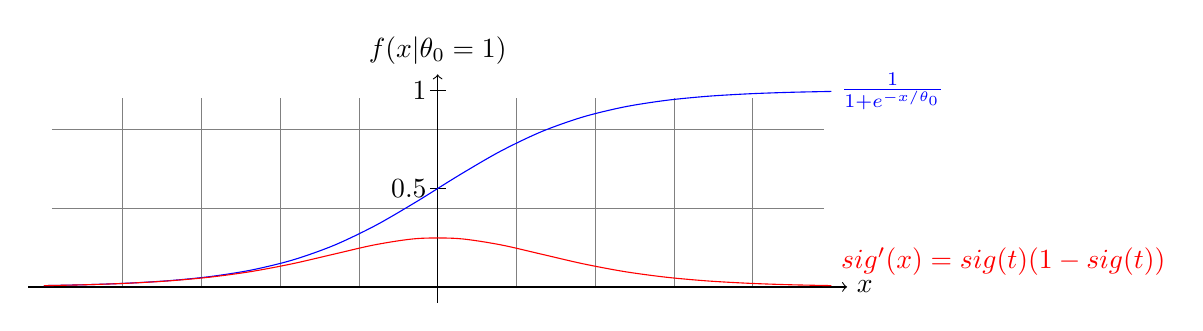
\begin{tikzpicture}[domain=-5:5, smooth, samples=20]
	\draw[very thin, color=gray] (-4.9,0.0) grid (4.9,2.4);

	\draw[->] (-5.2,0) -- (5.2,0) node[right] {$x$};
	\draw[->] (0,-0.2) -- (0,2.7) node[above] {$f(x|\theta_0=1)$};
	\draw (-0.1,2.5) --(0.1,2.5) node [left] {$1~$};
	\draw (-0.1,1.25) -- (0.1,1.25) node [left] {$0.5~$};

	\draw[color=blue] plot (\x,{2.5 / (1+exp(-\x))}) node[right] {$\frac{1}{1+e^{-x/\theta_0}}$};
	\draw[color=red]  plot (\x,{2.5 / (1+exp(-\x)) * (1-1/(1+exp(-\x)))}) node[above right] {$sig'(x)=sig(t)(1-sig(t))$};
\end{tikzpicture}


\caption{Sigmoid function}
\label{fig:sigmoid}
\end{figure}

%TODO: source?
If $K$ is the layer preceding layer $J$ then the input to the activation function of node $j$ in layer $J$ is the weighted sum of the outputs of Layer $K$.

\begin{align*}
I_j = \sum_{k=1}^{N_k}w_{jk}O_k
\end{align*}

\subsubsection{Forward Pass through a feedforward Neural Network\buchSeite{948}}
If an input vector $\mathbf{x}$ needs to be classified, a forward pass is calculated, hence the weights and biases must be known.
The outputs of layer 1 are the components of input vector $\mathbf{x}$
\[
  a_j(1)=x_j \qquad j = 1,2,\ldots,n_1
\]
where $n_1 = n$ is the dimensionality of $\mathbf{x}$.
The pre-activation of neuron $i$ in layer $l$ is then calculated
\[
  z_i(l) = \sum_{j=1}^{n_{l-1}} w_{ij}(l)a_j(l-1) + b_i(l) \qquad i=1,2,\ldots,n_l \qquad l=2,\ldots,L
\]
Then the output of neuron $i$ in layer $l$ is calculated by running the pre-activation through the activation function (usually ReLU)
\[
  a_i(l) = h(z_i(l)) \qquad i=1,2,\ldots,n_l
\]
The final output is then calculated with
\[
 a_i(L) = h(z_i(L)) \qquad i=1,2,\ldots,n_L
\]
where the activation function is usually a softmax (SM) function.\\
Note: softmax is not an element-wise function, hence the entire vector $\mathbf{z}$ needs to be fed into the SM function.

\paragraph{Matrix formulation\buchSeite{950}}
As it turns out a more efficient implementation can be achieved by using matrix notation.
Again, the outputs of layer 1 are the components of input vector $\mathbf{x}$
\[
  \mathbf{a}(1) = \mathbf{x}
\]
Given the proper definition of the weight matrix,
\[
  \mathbf{W}(l) =
  \begin{bmatrix}
    w_{11}(l) & w_{12}(l) & \ldots & w_{1n_{l-1}}(l) \\
    w_{21}(l) & w_{22}(l) & \ldots & w_{2n_{l-1}}(l) \\
    \vdots & \vdots & \ldots & \\
    w_{n_l1}(l) & w_{n_l2}(l) & \ldots & w_{n_ln_{l-1}}(l) \\
  \end{bmatrix}
\]
the pre-activations can be written as a matrix vector multiplication and a vector addition
\[
  \mathbf{z}(l) = \mathbf{W}(l)\mathbf{a}(l-1) + \mathbf{b}(l) \qquad l=2,3,\ldots,L
\]
Finally, the activation of the element-wise activation functions, such as ReLU and sigmoid can be written as (not true for sotmax)
\[
  \mathbf{a}(l) = h[\mathbf{z}(l)] =
  \begin{bmatrix}
    h(z_1(l)) \\
    h(z_2(l)) \\
    \vdots \\
    h(z_{n_l}(l)) \\
  \end{bmatrix}
\]


Usually the forward pass needs to be calculated for a mini-batch of input vectors.
For a mini-batch, the input vectors are concatenated column wise to create an $nxn_p$ matrix $\mathbf{X}$, where $n$ is the dimension of an input vector and $n_p$ is the number of input vectors in the mini-batch.
This concatenation then results in concatenated pre-activations and activations but else stays the same

\begin{table}[h]
	\begin{tabularx}{\textwidth}{lXl}
		\textbf{Step} & \textbf{Description} & \textbf{Equations} \\ \hline
		Step 1 & Input patterns & $\displaystyle\mathbf{A}(1) = \mathbf{X}$ \\
		Step 2 & Feedforward & $\displaystyle\text{For } l=2,\ldots,L, \text{ compute } \mathbf{Z}(l) = \mathbf{W}(l)\mathbf{A}(l-1) + \mathbf{B}(l) \text{ and } \mathbf{A}(l) = h(\mathbf{Z}(l))$ \\
		Step 3 & Output & $\displaystyle\mathbf{A}(L) = h(\mathbf{Z}(L))$ \\
		\hline
	\end{tabularx}
  \caption{Forward pass}
  \label{tab:forwardPass}
\end{table}

Note that $\mathbf{B}(l)$ contains $n_p$ columns of the bias vector $b(l)$, since it is the same bias vector at every input vector, $h()$ is applied element-wise and Step 3 is special for softmax since a normalization per column is needed, hence it is a column-wise function.


\subsubsection{Training by Backpropagation\buchSeite{953}}
Target is to minimize the total squared error between the desired responses
$r_q$ and the actual response $O_q$ in the output layer $Q$
\begin{align*}
	E = \frac{1}{2} \sum_{j=1}^{n_L}(r_j-a_j(L))^2
\end{align*}

Backpropagation is deriving the rate of change of $E$ with respect to the weights and biases in terms of quantities we can compute.
We can now update the network parameters using gradient descent
\begin{align*}
  w_{ij}(l) = w_{ij}(l) - \alpha \frac{\partial E(l)}{\partial w_{ij}(l)} = w_{ij}(l) - \alpha \delta_i(l)a_j(l-1)
\end{align*}
$\mathbf{w}$ is the weight vector, $\mathbf{b}$ the bias vector, $\alpha$ the correction increment, $E$ the error.

\paragraph{Matrix formulation\buchSeite{956}}
\begin{table}[h]
	\begin{tabularx}{\textwidth}{llX}
		\textbf{Step} & \textbf{Description} & \textbf{Equations} \\ \hline
		Step 1 & Input patterns & $\displaystyle\mathbf{A}(1) = \mathbf{X}$ \\
		Step 2 & Forward pass & $\displaystyle\text{For } l=2,\ldots,L, \text{ compute } \mathbf{Z}(l) = \mathbf{W}(l)\mathbf{A}(l-1) + \mathbf{B}(l) \text{; } \mathbf{A}(l) = h(\mathbf{Z}(l)) \text{;}\newline
    h'(\mathbf{Z}(l)) \text{; } \text{and } \mathbf{D}(l) = (\mathbf{A}(l) - \mathbf{R}) \odot h'(\mathbf{Z}(l))$ \\
		Step 3 & Backpropagation & $\displaystyle\text{For } l=L-1,L-2,\ldots,2, \text{ compute } \mathbf{D}(l) = (\mathbf{W}^T(l+1)\mathbf{D}(l+1)) \odot h'(\mathbf{Z}(l))$ \\
    Step 4 & Update weights and biases & $\displaystyle\text{For } l=2,\ldots,L, \text{ let } \mathbf{W}(l)=\mathbf{W}(l) - \alpha\mathbf{D}(l)\mathbf{A}^T(l-1),\newline
    \mathbf{b}(l) = \mathbf{b}(l) - \alpha\sum_{k=1}^{n_p}\pmb{\delta}_k(l), \text{ and } \mathbf{B}(l)= \underset{n_p \text{ times}}{\text{concatenate}}\{\mathbf{b}(l)\},\newline
    \text{where the } \pmb{\delta}_k(l) \text{ are the columns of } \mathbf{D}(l)$ \\
		\hline
	\end{tabularx}
\end{table}
Note that this table assumes identical element-wise activation functions everywhere and an MSE error function.
If the output activation function is a softmax and the error function is the cross entropy, then step 2 needs to change:
\begin{itemize}
  \item $\mathbf{A}(L) = \text{softmax}(\mathbf{Z}(l))$
  \begin{itemize}
    \item softmax is applied column-wise, since it is a function that takes a vector and returns a vector
  \end{itemize}
  \item $\mathbf{D}(L) = (\mathbf{A}(L) - \mathbf{R})$
  \begin{itemize}
    \item If the cross-entropy $L(\mathbf{a}(\mathbf{L}),\mathbf{r}) = \sum_i r_i \text{log}(\frac{1}{a(L)_i})$ is used as a loss function and $\mathbf{a}(\mathbf{L}) = \text{softmax}(\mathbf{z}(\mathbf{L}))$ is used to calculate $\mathbf{a}(\mathbf{L})$, then the gradient of the scalar loss function $L(\mathbf{a}(\mathbf{L}),\mathbf{r})$ with respect to the unnormalized log probabilites in the $\mathbf{z}(\mathbf{L})$ vector is the negative error vector $-\mathbf{e} = (\mathbf{a}(\mathbf{L}) - \mathbf{r})$
  \end{itemize}
\end{itemize}

\paragraph{Some facts about NN}
\begin{itemize}
\item Training with noisy data helps improving performance
\item Training with more patterns also
\item Single layer perceptron results in hyperplanes
\item Two layers result in open or closed convex regions
\item Three layers result in arbitrary (limited by the number of nodes) regions
\item More than three layers are never needed
\end{itemize}


\subsection{Deep Convolutional Neural Networks\buchSeite{964}}
The basic idea is that the NN finds its own set of of features at different abstraction levels and different resolution using convolution
\begin{itemize}
  \item Feature maps at different abstraction levels are created by learned filters and NOT by human based feature engineering
  \item The filters are the learned weights, hence, the weights are shared across the image and therefore much less weights need to be trained than in a fully connected NN
  \item The pooling (downsampling) reduces spatial resolution and also results in some invariance to feature translation while reducing the capacity and complexity of the NN
\end{itemize}
\begin{figure}[htp]
  \centering
  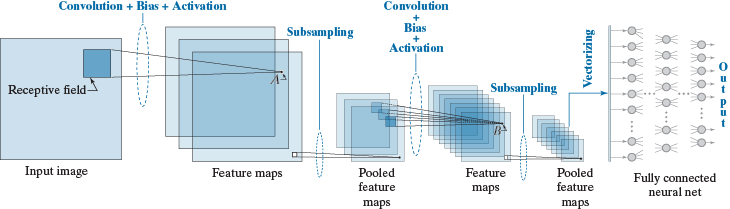
\includegraphics[width=\linewidth]{images/cnn.png}
  \caption{CNN, LeNet architecture}
  \label{fig:cnn}
\end{figure}

\subsubsection{Neural Computations in a CNN\buchSeite{971}}
The convolution value at any point $(x,y)$ is
\[
  w \star a_{x,y} = \sum_l \sum_k w_{l,k} a_{x-l,y-k}
\]
where $l$ and $k$ span the dimension of the kernel $w$.
Assume $w$ is a 3x3, then this expands to
\[
  w \star a_{x,y} = w_{1,1}a_{x-1,y-1} + w_{1,2}a_{x-1,y-2} + \ldots + w_{3,3}a_{x-3,y-3}
\]
Going from 2-D to indexing to 1-D indexing $i=3(l-1)+k$
\[
  w \star a_{x,y} = w_1a_1 + w_2a_2 + \ldots + w_9a_9 = \sum_{i=1}^{9} w_ia_i
\]
To get the usual NN summation for the pre-activation $z$, a bias is added
\[
  z = \sum_{j=1}^{9} w_ja_j + b = w \star a_{x,y} + b
\]
The activation is calculated by running the pre-activation through the activation function
\[
  a = h(z)
\]
\\

Consider a single pixel in a feature map, point $A$ in Fig. \ref{fig:cnn}.
Convolving the receptive field of the input image with the learned 2D filter weights and then adding a learned bias before running the result through an activation function, is identical to the steps performed in a fully connected NN.
What is different though is the fact, that the same learned weights/bias are used for all the pixels in a given feature map.\\

Consider a single pixel in a higher level feature map, point $B$ in Fig. \ref{fig:cnn}.
Since it is the result of convolving three pooled feature maps the calculations contain now the sum of three convolutions
\[
  w_{l,k}^{(1)} \star a_{x,y}^{(1)} + w_{l,k}^{(2)} \star a_{x,y}^{(2)} + w_{l,k}^{(3)} \star a_{x,y}^{(3)} = \sum_l \sum_k w_{l,k}^{(1)}a_{x-l,y-k}^{(1)} + \sum_l \sum_k w_{l,k}^{(2)}a_{x-l,y-k}^{(2)} + \sum_l \sum_k w_{l,k}^{(3)}a_{x-l,y-k}^{(3)}
\]
Nevertheless, each convolution can be written again as a simple sum over a new 1D index.
At the end the sum of these sums is augmented with a bias term and then run through an activation function.

\subsubsection{CNN Forward pass\buchSeite{973}}
Using a layer notation again, the pre-activation at a given pixel is
\[
  z_{x,y}(l) = \sum_l \sum_k w_{l,k}(l) a_{x-l,y-k}(l-1) + b(l) = w(l) \star a_{x,y}(l-1) + b(l)
\]
Hence the activation in a given layer $l$ at a given pixel is
\[
  a_{x,y}(l) = h(z_{x,y}(l))
\]
Note that the book now counts convolutional layers from 1 to $L_c$ which is a slight change in notation (so far, the layer count started at 2).
The convolutional layers start with the input image (possibly multi-dimensional) and stops with the multi-dimensional pooled features
\begin{align*}
  a_{x,y}(0) = \{\text{values of pixels in the input image}(s)\} \\
  a_{x,y}(L_c) = \{\text{values of pooled features in last layer of the CNN}\}
\end{align*}

Pooling layers have no parameters but are needed to reduce the spatial resolution.
For the derivation, we assume that no pooling layers are used, which results in
\begin{table}[h]
	\begin{tabularx}{\textwidth}{llX}
		\textbf{Step} & \textbf{Description} & \textbf{Equations} \\ \hline
		Step 1 & Input images & $\displaystyle a(0) = \text{ the set of image pixels in the input to layer 1}$ \\
		Step 2 & Forward pass & $\displaystyle\text{For each neuron corresponding to location } (x,y) \text{ in each feature map in layer } l \text{ compute:}\newline
    z_{x,y}(l) = w(l) \star a_{x,y}(l-1) + b(l) \text{ and } a_{x,y}(l) = h(z_{x,y}(l)) \text{; } l=1,2,\ldots,L_c$ \\
		\hline
	\end{tabularx}
\end{table}

The fully connected NN at the end of the last convolutional layer is identical to the ones already covered, see Table \ref{tab:forwardPass}.

\subsubsection{CNN Backpropagation\buchSeite{974}}
Since the forward pass is very similar to a fully connected NN, the same is expected for backpropagation:
\begin{align*}
  \frac{\partial E}{\partial b(l)} &= \sum_x \sum_y \delta_{x,y}(l) \\
  w_{l,k}(l) &= w_{l,k}(l) - \alpha \frac{\partial E}{\partial w_{l,k}} = w_{l,k}(l) - \alpha \delta_{l,k}(l) \star \text{rot180}(a(l-1)) \\
  b(l) &= b(l) - \alpha \frac{\partial E}{\partial b(l)} = b(l) - \alpha \sum_x \sum_y \delta_{x,y}(l)
\end{align*}
In the forward pass, the pooling reduced the spatial resolution.
Hence in backpropagation, the resolution needs to be increased.
\begin{itemize}
  \item For average pooling this is achieved by pixel replication, since each high res pixel contributed equally for the low res pixel (e.g., kron(temp,ones(2,2)/4);)
  \item For max pooling this is achieved by remembering which high res pixels won and copy the low res values to those pixels while setting the loser pixels to zero
\end{itemize}
\begin{table}[h]
	\begin{tabularx}{\textwidth}{llX}
		\textbf{Step} & \textbf{Description} & \textbf{Equations} \\ \hline
		Step 1 & Input images & $\displaystyle a(0) = \text{ the set of image pixels in the input to layer 1}$ \\
		Step 2 & Forward pass & $\displaystyle\text{For each neuron corresponding to location } (x,y) \text{ in each feature map in layer } l\newline
    \text{compute: } z_{x,y}(l) = w(l) \star a_{x,y}(l-1) + b(l) \text{ and } a_{x,y}(l) = h(z_{x,y}(l)) \text{; } l=1,2,\ldots,L_c$ \\
    Step 3 & Backpropagation & $\displaystyle\text{For each neuron in each feature map in layer } l \text{ compute:}\newline
    \delta_{x,y}(l) = h'(z_{x,y}(l))[\delta_{x,y}(l+1) \star \text{rot180}(w(l+1))] \text{; } l=L_c-1,L_c-2,\ldots,1$ \\
    Step 4 & Update parameters & $\displaystyle\text{Update the weights and bias for each feature map using }\newline
    w_{l,k}(l) = w_{l,k}(l) - \alpha\delta_{l,k}(l) \star \text{rot180}(\alpha(l-1)) \text{ and } b(l)=b(l) - \alpha\sum_x\sum_y\delta_{x,y}(l) \text{; }\newline
    l=1,2,\ldots,L_c $ \\
		\hline
	\end{tabularx}
\end{table}
